% !TEX TS-program = pdfLaTeX+shellescape
% !TEX encoding = UTF-8 Unicode

\documentclass[class=beamer,tikz]{standalone}
\setbeamertemplate{navigation symbols}{} % For delete the navigation symbols
\usepackage{pgfplots}
\pgfplotsset{compat=1.17}

\begin{document}
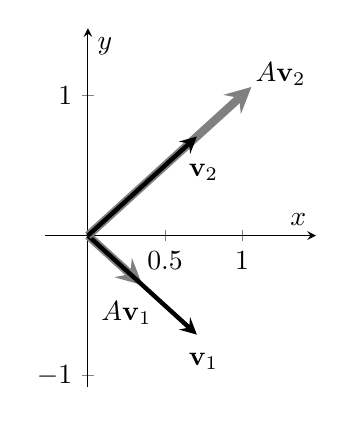
\begin{tikzpicture}[baseline]
\begin{axis}[
scale=0.8,xmin=-0.28,xmax=1.48,ymin=-1.08,ymax=1.48,
legend style={at={(axis cs: 1,0)}, anchor=south east},
unit vector ratio = {1,1},
axis lines = middle,
xlabel = {$x$}, ylabel = {$y$}, % axis labels
]
\draw[line width = 3,->,>=stealth,color=gray] (axis cs:0,0) -- (axis cs:0.35355,-0.35355);
\draw[ultra thick,->,>=stealth] (axis cs:0,0) -- (axis cs:0.7071,-0.7071);
\draw[line width = 3,->,>=stealth,color=gray] (axis cs:0,0) -- (axis cs:1.06066,1.06066);
\draw[ultra thick,->,>=stealth] (axis cs:0,0) -- (axis cs:0.7071,0.7071);
\node at (axis cs: 0.75,-0.9) {$\mathbf{v}_1$};
\node at (axis cs: 0.25,-0.55) {$A\mathbf{v}_1$};
\node at (axis cs: 0.75,0.45) {$\mathbf{v}_2$};
\node at (axis cs: 1.25,1.15) {$A\mathbf{v}_2$};
%\addplot[black,mark=none]gnuplot{y=x};
%\addplot[black,mark=none]gnuplot{"data_bubble60h.txt" index 432};
%\addplot[magenta,mark=none]gnuplot{"data_bubble60zeta.txt" index 432};
%\legend{bubble height $h$, liquid height $\zeta$}
\end{axis}
\end{tikzpicture}
\end{document}